\documentclass[14pt  aspectratio = 169]{beamer}
\usetheme {Frankfurt}
\usecolortheme{orchid}
\usepackage{graphicx}
\usepackage{listings}

\title{ Nonogram Bot }
\subtitle { \textit {Puzzle Your Way to Pixel Perfection}}
\date {\today}

% Begin Document
\begin{document}


 % Title slide
\begin{frame}
  \titlepage
\end{frame}

% Introduction
\begin{frame} 
   \frametitle {Introduction}
       \begin{center}
           \textbf{What are nonograms?}  
       \end{center}
       \newline{Nonograms are picture logic puzzles in which cells in a grid must be colored or left blank according to numbers at the side of the grid to reveal a hidden pixel art-like picture.}
\end{frame}

% Task 
\begin{frame}       
\frametitle{Objective}
 \begin{center}
       \textbf {Task}
\end{center}
        \newline {We are aiming at coming up with a} \emph{Nonogram Bot} {which takes input from the user which includes the clues of the rows and columns. The bot is designed to return a solved nonogram unraveling the hidden pixel art.}
\end{frame}       


%Nonogram puzzles examples
\begin{frame}
    \frametitle {Nonogram puzzles}
     \begin{figure}
    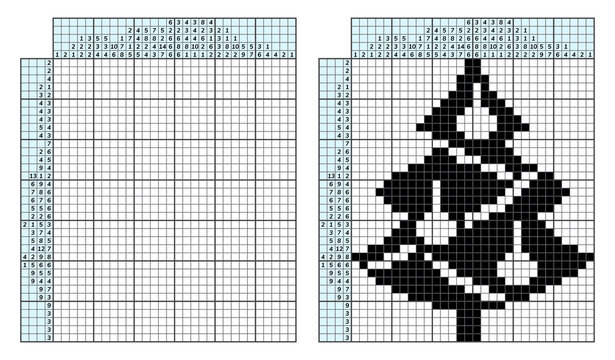
\includegraphics[width=0.5\textwidth]{/Users/lakshmipathibojja/Desktop/beamer latex/nonogram_one.jpeg}
    \caption{Here are a few nonogram examples}
  \end{figure}
\end{frame}


% Rules 
\begin{frame}
    \frametitle {Game Rules}
        \begin{itemize}
           \item [Grid]{You start with a rectangular grid consisting of rows and columns. Each cell in the grid can be either filled or left blank.}
           \item [Clues] {For each row and column, there are numeric clues given at the edges of the grid. These clues indicate the lengths of consecutive filled cells in that row or column. The order of the clues corresponds to the order of the filled cells.}
           \item [Solve]{Solving a nonogram requires logical deduction. By analyzing the clues and the filled cells, you can determine which cells are definitely filled or definitely empty. The filled cells will eventually form a picture.}
           \item [Marking]{ To keep track of the cells you have solved, you can use symbols to mark them.A filled cell is marked with an X , and an empty cell is represented by \_ (underscore)}
       \end{itemize}
\end{frame}


% styling the listings package
\lstset{language=Python, % Set the programming language
        basicstyle=\ttfamily\small, % Set the font style
        keywordstyle=\color{blue}, % Set keyword color
        commentstyle=\color{green!40!black}, % Set comment color
        stringstyle=\color{purple}, % Set string color
        showstringspaces=false, % Don't show spaces in strings
        breaklines=true, % Allow line breaks
        frame=single, % Add a frame around the code
        numbers=left % Show line numbers
}

% including the code file #1
\begin{frame}[fragile]
  \frametitle{empty\_ grid\_creation.py }
  \begin{lstlisting}
    EMPTY = "o"
    FILLED = "x"
    def empty_grid(grid_size: int) -> list[list[str]]:
        empty_grid = []
        for row in range(grid_size):
            empty_grid.append([EMPTY] * grid_size)
        return empty_grid

  \end{lstlisting}

\end{frame}

% including the code #2
\begin{frame}[fragile]
  \frametitle{numbers\_creation.py }
  \begin{lstlisting}
    def cross_pattern() -> list[list[str]]:
	all_row_clues = ["3", "2 2", "1 1", "2 2", "3"]
	all_column_clues = ["3", "2 2", "1 1", "2 2", "3"]
	return [all_row_clues, all_column_clues]


  \end{lstlisting}

\end{frame}






\end{document}